\documentclass[12pt]{report}

\usepackage{multicol}

\usepackage{geometry}
\geometry{margin=1in}

% Boxes
\usepackage{tcolorbox}
\newtcolorbox{codebox}{
	colback=gray!5!white,
	colframe=gray!30!white,
	boxsep=1pt,
	top=0pt,
	bottom=0pt,
	boxrule=0.1pt
}

\begin{document}

\section*{Introduction to Git for Bioinformaticians - Commands}

\subsubsection*{Syllabus}

\begin{itemize}
	\item Angular brackets (\verb$<>$) - Input path/string/...
	\item Square brackets (\verb$[]$) - Optional argument
\end{itemize}

%\begin{multicols}{1}

\pagenumbering{gobble}

\subsubsection{1. Introduction to version control}

\verb$git <command> -h              $ \hspace*{25pt} Short help\\
\verb$git <command> --help          $ \hspace*{25pt} Open man-page for command

\subsubsection{2. Introduction to the file system}

\verb$git init                      $ \hspace*{25pt} Initialize new repository \\
\verb$git add [-A] <path>           $ \hspace*{25pt} Stage file-edit (create, edit, remove) \\
\verb$git commit [-m <message>]     $ \hspace*{25pt} Commit staged files \\
\verb$git status                    $ \hspace*{25pt} Get current status for repository

\subsubsection{3. Investigating your history}

\verb$git log [--oneline]           $ \hspace*{25pt} Short help\\
\verb$git checkout <id/head/tag>    $ \hspace*{25pt} Move \verb$HEAD$ to specified object \\
\verb$git diff <id1> [<id2>]        $ \hspace*{25pt} Print differences between targets

\subsubsection{4. Branches}

\verb$git branch <name> [<target>]  $ \hspace*{25pt} Create new branch \\
\verb$git branch -d <name>          $ \hspace*{25pt} Delete branch \\
\verb$git merge <branch name>       $ \hspace*{25pt} Merge target branch into current branch

\subsubsection{5. Remote repositories}

\verb$git clone <URL>               $ \hspace*{25pt} Clone target repository \\
\verb$git fetch                     $ \hspace*{25pt} Get information about remote updates \\
\verb$git pull                      $ \hspace*{25pt} Retrieve updates made to remote \\
\verb$git push                      $ \hspace*{25pt} Send changes to remote \\
\verb$git push                      $ \hspace*{25pt} Send changes to remote \\
\verb$git remote -v                 $ \hspace*{25pt} Print remote URLs (fetch and push) \\
\verb$git remote add origin <path>  $ \hspace*{25pt} Add path to remote \\
\verb$git push --set-upstreams origin master$ \hspace*{10pt} Push and establish connection to remote

\subsubsection{6. Version control for bioinformaticians}

\verb$git rm --cached <path>        $ \hspace*{25pt} Remove file from repo (not from file tree) \\
\verb$git tag -a <tag-name> -m <message>$ \hspace*{0pt} Send changes to remote \\
\verb$git push origin <tag>         $ \hspace*{25pt} Push tag to remote

\newpage

\section*{.gitignore patterns}

Used to keep files within file tree of repository, without tracking them in the repository itself. \\\\
\verb$<file path>                   $ \hspace*{25pt} Ignore specific file \\
\verb$<folder path>                 $ \hspace*{25pt} Ignore specific directory with sub-files \\
\verb$*.<suffix>                    $ \hspace*{25pt} Ignore all files with suffix \\
\verb$**<folder-name>               $ \hspace*{25pt} Ignore all folder with given name \\

\section*{Common use patterns}

\subsection*{Basic usage}

\begin{codebox}
\begin{verbatim}
$ git init                          # Initialize directory
$ echo "Content" > my_file.txt      # Add files
$ git add my_file.txt               # Stage changes
$ git commit -m "Adding a file"     # Commit staged changes
\end{verbatim}
\end{codebox}

\subsection*{Checking out the history}

\begin{codebox}
\begin{verbatim}
$ git log                           # Print the history of commits
$ git checkout 56basda              # Move HEAD to commit ID
$ git checkout master               # Return to master when done
\end{verbatim}
\end{codebox}

\subsection*{Create branch and merge branch}

\begin{codebox}
\begin{verbatim}
$ git branch my_branch              # Create new branch
$ git checkout my_branch            # Switch branch to the new branch
... commit some changes
$ git checkout master               # Return to master
... commit some changes to master
$ git merge my_branch               # Merge branch back into master
$ git branch -d my_branch           # Remove unused branch
\end{verbatim}
\end{codebox}

\subsection*{Set up remote}

If you have a repository for which you want to set up the remote. If you want to retrieve an existing remote, use \verb$git clone$. \\\\
\begin{codebox}
\begin{verbatim}
$ git remote add origin https://GitHub/Jakob37/MyRepo # Add remote URL
$ git push --set-upstreams origin master              # Push and initiate
\end{verbatim}
\end{codebox}

\newpage

\section*{Overview of the different stages in Git}

\begin{figure}[h!]
	\centering
	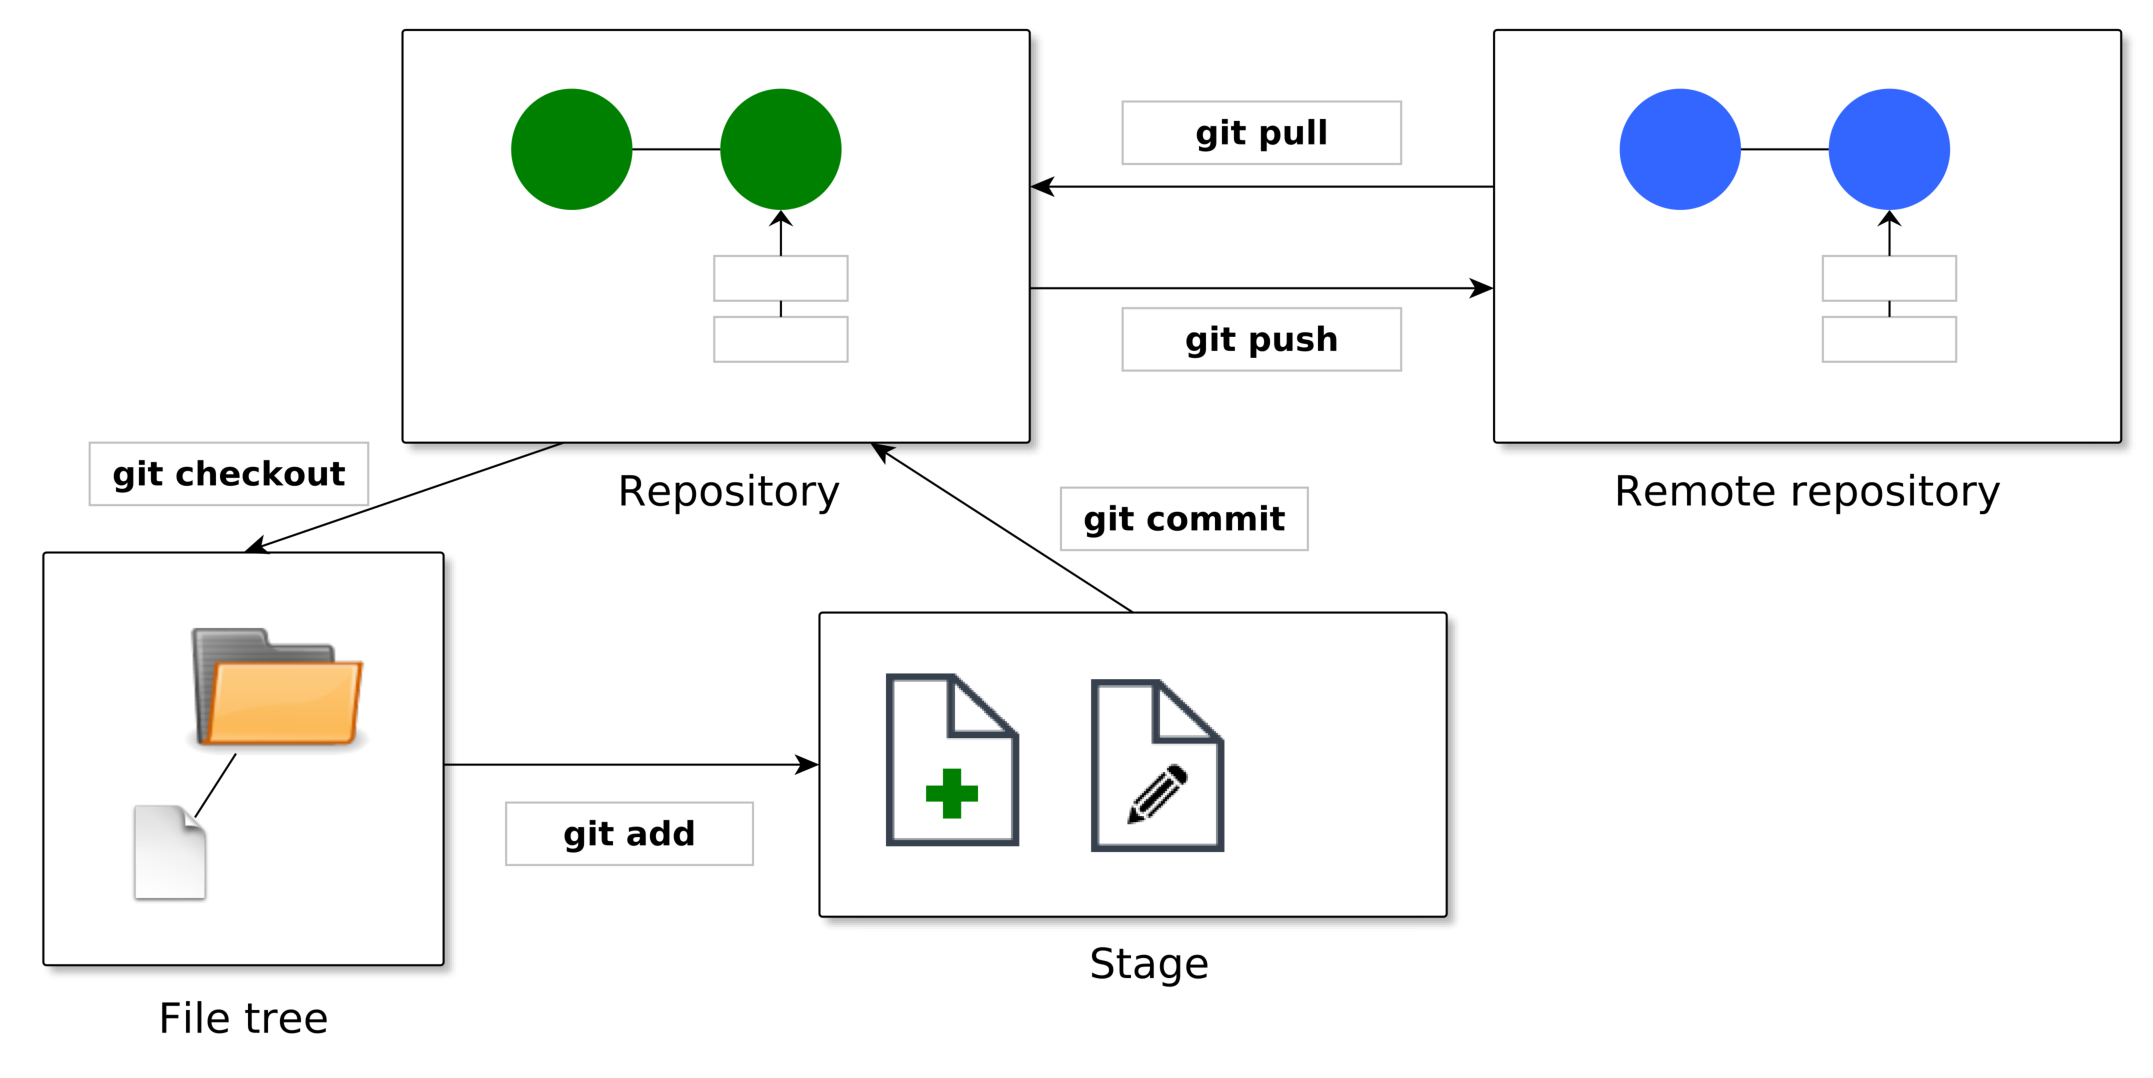
\includegraphics[width=1.0\textwidth]{../visualizations/chapter5/51_stages_including_remote.pdf}
	\label{fig:all_stages_visualized}
\end{figure}

%\end{multicols}

\end{document}